%===============================================================================
% $Id: ifacconf.tex 19 2011-10-27 09:32:13Z jpuente $  
% Template for IFAC meeting papers
% Copyright (c) 2007-2008 International Federation of Automatic Control
%===============================================================================
\documentclass[a4paper]{ifacconf}

\usepackage{graphicx,amsmath,url}      % include this line if your document contains figures
\usepackage[round]{natbib}             % required for bibliography
%===============================================================================


% ===============================================================
% Choose the language of the manuscript.
% If in English, choose 
% \def\portugues{0} 
%
% If in Portuguese or Spanish, choose
% \def\portugues{1} 
%
% Note that, if you are writing in Spanish, you need additional 
% adjusts in some parts of the text, which have been put in Portuguese only.
\def\portugues{1} 
% ===============================================================

% If the above line is commented, it is assumed manuscript in English:
\ifx\portugues\undefined
\def\portugues{0}
\fi


\if\portugues0
   \usepackage[english]{babel}
  \else
   \usepackage[spanish,brazil,english]{babel}
\fi

  

\usepackage[T1]{fontenc}
%\usepackage{inputenc}

\usepackage[utf8]{inputenc}

\usepackage{ae}


\if\portugues1
% =====================================================================
% =====================================================================
% If the manuscript is in Spanish, please change the texts adequatelly.
% You may also add other definitions in this part.
 \newtheorem{teorema}[thm]{{\em Teorema}}{ }
 \newtheorem{lema}[thm]{{\em Lema}}{ }
 \newtheorem{corolario}[thm]{{\em Corolário}}{ }
 \newenvironment{prova}{{\bf Prova.}}{ }
% ===============================================================
\fi

\begin{document}
	
	
\if\portugues1

% =====================================================================
% =====================================================================
% USE THIS PART IF THE TEXT IS IN PORTUGUES OR SPANISH
% =====================================================================
% If the manuscript is in Spanish, please change the texts adequately.
% =====================================================================
% 
\selectlanguage{brazil}
	
\begin{frontmatter}

\title{Uma abordagem de Aprendizado por Reforço Online para Robôs Seguidores de Linha} 
% Title, preferably not more than 10 words.

%\thanksref{footnoteinfo}
%\thanks[footnoteinfo]{Reconhecimento do suporte financeiro deve vir nesta nota de rodapé.}


\author[First]{Mateus S. Franco} 
\author[Second]{Sérgio R. B. Santos}

\address[First]{Instituto de Ciência e Tecnologia, Universidade Federal de São Paulo, SP, (e-mail: mateus.franco@unifesp.br).}
\address[Second]{Instituto de Ciência e Tecnologia, Universidade Federal de São Paulo, SP, (e-mail: sergio.ronaldo@unifesp.br).}



\selectlanguage{english}
\renewcommand{\abstractname}{{\bf Abstract:~}}
\begin{abstract}                % Abstract of not more than 250 words.
Several methods had emerged with evolution of Machine Learning (ML). Among them is the Reinforcement Learning (RL) in which the agent learns how to choose the best action to maximize the amount of received rewards through direct interactions with the environment. This study presents the design and development of a terrestrial line-follower robotic platform using an online RL approach. Implenting the Q-learning algorithm the robot learned how to control the speed and direction of its movement to follow lines as presented in two different learning processes.


\vskip 1mm% não altere esse espaçamento
\selectlanguage{brazil}
{\noindent \bf Resumo}:  Diversos métodos de \emph{Machine Learning} (ML) surgiram com a evolução deste campo. Dentre eles está o \emph{Reinforcement Learning} (RL), do inglês Aprendizado por Reforço, um método que permite ao agente descobrir qual a melhor ação a ser tomada de modo a maximizar as recompensas recebidas através de interações diretas com o ambiente. Este trabalho apresenta o projeto e desenvolvimento de uma plataforma robótica terrestre do tipo seguidor de linha que utiliza uma abordagem online de RL. Implementando o algoritmo Q-learning, o robô aprendeu a controlar a velocidade e a direção do seu movimento para seguir linhas, conforme apresentados em dois estudos de caso com configurações distintas de aprendizado.
\end{abstract}

\selectlanguage{english}


\begin{keyword}
Reinforcement Learning; Online Learning; Q-learning; Line-follower; PID Controller; Computer Vision;

\vskip 1mm% não altere esse espaçamento
\selectlanguage{brazil}
{\noindent\it Palavras-chaves:} Aprendizado por Reforço; Aprendizado Online; Q-learning; Seguidor de Linha; Controlador PID; Visão Computacional
\end{keyword}


\selectlanguage{brazil}


\end{frontmatter}
\else
% ===============================================================
% ===============================================================
% USE THIS PART IF THE TEXT IS IN ENGLISH
% ===============================================================
% ===============================================================
% 

\begin{frontmatter}

\title{Style for SBA Conferences \& Symposia: Use Title Case for
  Paper Title\thanksref{footnoteinfo}} 
% Title, preferably not more than 10 words.

\thanks[footnoteinfo]{Sponsor and financial support acknowledgment
goes here. Paper titles should be written in uppercase and lowercase
letters, not all uppercase.}

\author[First]{First A. Author} 
\author[Second]{Second B. Author, Jr.} 
\author[Third]{Third C. Author}


\address[First]{Faculdade de Engenharia Elétrica, Universidade do Triângulo, MG, (e-mail: autor1@faceg@univt.br).}
\address[Second]{Faculdade de Engenharia de Controle \& Automação, Universidade do Futuro, RJ (e-mail: autor2@feca.unifutu.rj)}
\address[Third]{Electrical Engineering Department, 
   Seoul National University, Seoul, Korea, (e-mail: author3@snu.ac.kr)}
   
\renewcommand{\abstractname}{{\bf Abstract:~}}   
   
\begin{abstract}                % Abstract of not more than 250 words.
These instructions give you guidelines for preparing papers for IFAC
technical meetings. Please use this document as a template to prepare
your manuscript. For submission guidelines, follow instructions on
paper submission system as well as the event website.
\end{abstract}

\begin{keyword}
Five to ten keywords, preferably chosen from the IFAC keyword list.
\end{keyword}

\end{frontmatter}
\fi

%===============================================================================
%===============================================================================
%===============================================================================


\section{Introdução}


As técnicas clássicas de projeto de controladores envolvem a obtenção de um modelo matemático do sistema a ser controlado, que nada mais é do que um conjunto de expressões que descrevem e modelam o seu comportamento. Esta etapa tende a ter uma complexidade que varia de acordo com o tipo de sistema e com as condições estabelecidas para a derivação dos modelos, podendo levar a modelos matemáticos extremamente complexos, mesmo que lineares, e não necessariamente precisos. A complexidade de modelos não-lineares tende a ser maior, entretanto, qualquer sistema não-linear pode ser linearizado para uma certa condição de operação, que é definida durante a linearização.

Um tipo de controlador amplamente utilizado devido à sua simplicidade de otimização e implementação é o controlador Proporcional-Integral-Derivativo (PID). Este controlador gera uma saída de controle proporcional ao erro entre o estado desejado e o estado atual (ganho proporcional), levando em consideração também a taxa de variação do valor (ganho derivativo) e o erro acumulado ao longo do tempo (ganho integral). O PID é um controlador geralmente empregado em sistemas lineares, também podendo ser empregado em alguns sistemas não-lineares \cite{nonLinearPID}  desde que algumas condições de linearização sejam estabelecidas em troca de um comportamento sub ótimo quando fora dessas condições \cite{pid_autotune_relay, pid_engine_tuning,embarcados_pid_1}.

O \emph{Reinforcement Learning} (RL), do inglês, Aprendizado por Reforço, pode ser adotado como um método de otimização em aplicações onde se deseja solucionar uma variedade de problemas de controle e planejamento em que os modelos dos sistemas não estão disponíveis a priori, aprendendo estratégias de controle adequadas, uma vez que tem a convergência garantida \cite{ql_pid_robotics,intro_to_rl,rl_rob_survey,ql_pid_robotics}.

No RL, o agente aprende por meio da interação direta com o ambiente, através de recompensas na forma de reforços positivos ou negativos, sinalizado ao agente se a ação tomada foi correta ou incorreta, respectivamente. O objetivo do agente sempre será acumular o máximo de reforço possível \cite{ql_pid_robotics,intro_to_rl,rl_rob_survey,ql_pid_robotics}.

Este tipo de abordagem possui um grande potencial no âmbito da robótica móvel, uma vez que robôs móveis são classificados como sistemas não-lineares cujo comportamento possui um elevado acoplamento e grau de incerteza associada à determinação dos estados, que são obtidos através da amostragem de sensores. Uma modelagem matemática rigorosa deste sistema geralmente leva a expressões e soluções complexas, de modo que um controlador simples como o PID não funcionaria de forma adequada. Utilizando uma abordagem \textit{online} de Aprendizado por Reforço, é possível fazer com que o robô encontre o ajuste adequado a partir da interação direta com o ambiente, obtendo um controlador que compreende o acoplamento e a não-linearidade, fatores usualmente desconsiderados em virtude das simplificações numa modelagem utilizando controle clássico \cite{ql_pid_robotics}.

O RL pode ser utilizado para resolver diversos problemas de otimização no contexto de robótica móvel. Tomando como exemplo o robô seguidor de linha, que possui como tarefa navegar em um ambiente seguindo uma trajetória que é determinada por uma linha na superfície em que se movimenta. Este tipo de abordagem permite otimizar o controlador de velocidade angular dos motores que tracionam as rodas e também na determinação das velocidades necessárias de cada um dos motores, de modo que o robô sempre se mantenha em cima da linha, com o menor desvio possível. Este tipo de robô possui diversas aplicações industriais, como o transporte de mercadorias numa fábrica, e acadêmicos, como o estudo de algoritmos de controle e metodologias de programação \cite{path_plan_pid,lf_line_sens_pos}.


\section{Formulação do Problema}

A otimização da trajetória do robô é um dos problemas que podem ser resolvidos no caso do robô seguidor de linha aplicando o RL. Quanto menos o robô se desvia da trajetória definida pela linha, menor é o erro de posição entre o robô e a linha e, consequentemente, menor o tempo que o robô gasta para percorrer o circuito. Neste caso, por meio das interações, o RL irá aprender qual é a melhor combinação de velocidades de rotação dos motores para que o robô se mantenha o mais próximo possível da linha, condição de maiores recompensas.

O motor de corrente contínua utilizado na maioria dos robôs se trata de um sistema não-linear, cuja modelagem rigorosa leva à expressões extremamente complexas. A otimização através do RL torna possível a obtenção de controladores ótimos e consequentemente um melhor controle de trajetória. No caso do controle de trajetória, o aprendizado por reforço permite que o robô aprenda a determinar sua melhor velocidade e direção a partir da posição relativa à linha, que é obtida através dos seus sensores.

\subsection{Robótica Móvel e Robôs Seguidores de Linha}

A Robótica Móvel é a área da robótica que estuda robôs e seus mecanismos de locomoção. Ao longo dos anos, diversas formas de implementar a mobilidade em plataformas robóticas foram desenvolvidas, o que criou uma ampla variedade de formas de locomoção, como por exemplo, robôs aéreos, terrestres e aquáticos. \cite{intro_to_auto_robots}. 

A precisão com a qual o robô móvel consegue seguir um trajeto está intimamente relacionada ao método utilizado para aferir a posição da linha e aos controladores que irão converter esta informação em uma ação. Para um seguidor de linha, o método para determinar a posição da linha e os controladores utilizados estão intimamente relacionados à precisão com a qual o robô consegue seguir a linha. 

No caso de robôs que utilizam sensores de reflectância, a quantidade de sensores determina o grau de discretização da escala de posições da linha. Uma quantidade maior de sensores possibilita gerar uma escala com um grau de discretização maior do que uma quantidade menor. O algoritmo utilizado no controle de orientação e velocidade também possui grande influência no comportamento geral do robô e na sua eficiência \cite{path_plan_pid,lf_line_sens_pos}.

\subsection{Modelagem Cinemática de Robôs com Duas Rodas}

O estudo cinemático de um robô permite estabelecer um modelo matemático que descreve o seu comportamento mecânico, permitindo o desenvolvimento de robôs que sejam adequados às tarefas e ajudando a projetar controladores de baixo nível eficientes. A partir deste modelo, é possível estabelecer o espaço de trabalho, que se trata basicamente do conjunto de pontos que um robô pode alcançar a partir de sua posição atual. 

Ao longo desta análise, o robô será modelado como um corpo rígido se movimentando no plano horizontal, que dá um total de três graus de liberdade, ou em inglês, \textit{Degrees of Freedom} (DoF), para descrever o seu movimento: dois referentes à posição no plano e um terceiro referente à orientação com relação ao eixo vertical, que é ortogonal ao plano de movimentação conforme observado na Figura~\ref{fig:mod_cin} e na Equação~\eqref{eq:dof} \cite{intro_to_auto_robots}.

\begin{figure}
\begin{center}
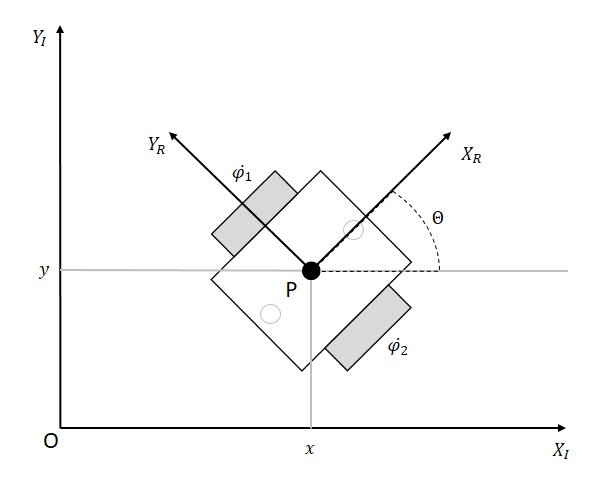
\includegraphics[scale=0.5]{Figuras/mod_cin.png}
\caption{Referenciais global e local para o modelo.}
\label{fig:mod_cin}
\end{center}
\end{figure}

\begin{equation}\label{eq:dof}
\xi_{I} = \begin{bmatrix}
x \\
y \\
\theta
\end{bmatrix}
\end{equation}

A partir desta equação básica e da aplicação de operações algébricas, é possível estabelecer a expressão matemática da Equação~\eqref{eq:mod_mov} que permite calcular os parâmetros de posição e movimento relativos ao referencial inercial, tomando como base a geometria do robô representada pela distância \emph{l} entre as rodas, de raio \emph{r}, e suas respectivas velocidades angulares. Este modelo encontra-se ilustrado na Figura~\ref{fig:mod_mov}.

\begin{figure}
\begin{center}
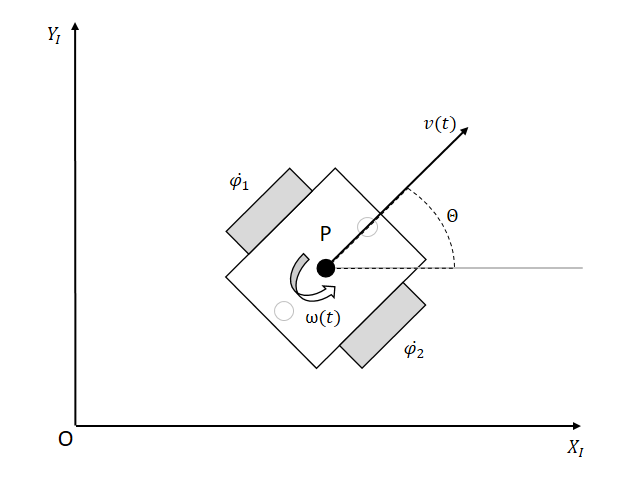
\includegraphics[scale=0.5]{Figuras/mod_mov.png}
\caption{Modelo do robô de duas rodas utilizando o referencial inercial.}
\label{fig:mod_mov}
\end{center}
\end{figure}

\begin{equation} \label{eq:mod_mov}
\dot{\xi_{I}} =
\begin{bmatrix}
\dot{x} \\
\dot{y} \\
\dot{\theta}
\end{bmatrix}=f(l,r,\theta,\dot{\varphi}_{1},\dot{\varphi}_{2}) 
\end{equation}

\subsection{Controlador PID de Baixo Nível}

O controlador Proporcional-Integral-Derivativo (PID) é um controlador amplamente utilizado pela sua simplicidade e bom desempenho para um grande número de aplicações, como por exemplo controle de temperatura de fornos, controle de velocidade, posição, dentre outros. O controlador PID é um sistema de malha fechada, ou seja, a saída de controle é calculada tomando como base o valor desejado e a leitura retornada pelos sensores \cite{pid_autotune_relay, pid_engine_tuning,embarcados_pid_1}.

O primeiro é o Termo Proporcional ($P$), que consiste na regulação da saída de forma proporcional ao erro, sendo assim, quanto maior o erro, mais intensa é a saída de controle. \cite{pid_autotune_relay,embarcados_pid_1}.

O segundo é o Termo Integral ($I$), que possui o ganho integral $K_{I}$ e atua diretamente na eliminação do chamado erro de estado estacionário, que acontece quando o sistema atinge uma condição de estabilidade sem atingir o \emph{setpoint} desejado \cite{pid_autotune_relay,embarcados_pid_1}.

O terceiro é o Termo Derivativo ($D$), com ganho $K_{D}$, que basicamente compara o erro atual com o erro da última leitura realizada, possuindo um efeito capaz de atenuar o sobressinal causado pelas ações proporcional e integral. \cite{pid_autotune_relay,embarcados_pid_1}.

Cada um destes termos e seus respectivos ganhos causam possuem efeitos colaterais. O Termo Integral e o Termo Proporcional quando em excesso podem fazer com que o controlador produza sobressinal enquanto o Termo Derivativo pode induzir uma maior demora no alcance do regime estacionário. 

A Equação~\eqref{eq:pid_ana} e a Figura~\ref{fig:pid_tempo} apresentam, respectivamente, uma forma de descrever o controlador PID no domínio do tempo contínuo e a sua representação em diagrama de blocos. A partir desta equação, é possível obter a Equação~\eqref{eq:pid_dig} seu equivalente em tempo discreto.

\begin{equation} \label{eq:pid_ana} 
u(t) = K_P\varepsilon(t)+K_I\int\varepsilon(t)\mathrm{d}x+K_D\varepsilon(t)/\mathrm{d}x
\end{equation}

\begin{equation} \label{eq:pid_dig} 
u[n] = K_{P}\varepsilon[n] + K_{D}(\varepsilon[n]-\varepsilon[n-1])+K_{I}(\varepsilon[n]+\varepsilon[n-1])
\end{equation}

\begin{figure}
\begin{center}
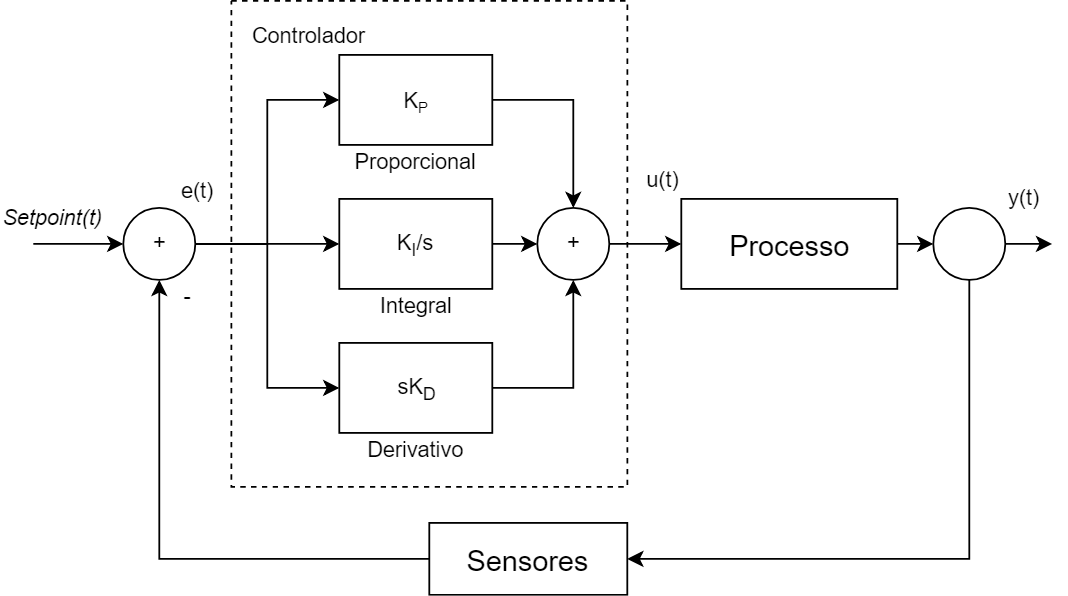
\includegraphics[scale=0.22]{Figuras/controlador_pid.png}
\caption{Diagrama de blocos de uma implementação padrão do Controlador PID.}
\label{fig:pid_tempo}
\end{center}
\end{figure}

\subsection{Visão Computacional}

Visão Computacional, em inglês \textit{Computer Vision} (CV), é uma área da ciência da computação que inclui uma série de recursos para adquirir, processar, analisar e entender imagens de modo semelhante à visão humana, sendo utilizada para tarefas como reconhecimento e classificação de objetos, ou detecção e análise de movimentos \cite{comp_vis}.

No âmbito de software, existem várias formas de implementar visão computacional em sistemas robóticos. Uma delas é utilizando uma biblioteca chamada OpenCV, que é uma biblioteca de código aberto desenvolvida inicialmente na Rússia e que traz um pacote repleto de métodos úteis à visão computacional incluindo o benefício de ser multiplataforma, podendo ser integrado em vários sistemas operacionais como Windows e sistemas baseados em Unix, utilizando linguagens de programação como C/C++, Java e Python \cite{comp_vis,ocv_ref}.



\subsection{Aprendizado por Reforço (RL) e Q-learning}


\section{Desenvolvimento}


\section{Resultadoos}


\section{Conclusão}




\section*{Agradecimentos}


\bibliography{ifacconf}             % bib file to produce the bibliography
                                                     % with bibtex (preferred)
                                                   
%\begin{thebibliography}{xx}  % you can also add the bibliography by hand

%\bibitem[Able(1956)]{Abl:56}
%B.C. Able.
%\newblock Nucleic acid content of microscope.
%\newblock \emph{Nature}, 135:\penalty0 7--9, 1956.

%\bibitem[Able et~al.(1954)Able, Tagg, and Rush]{AbTaRu:54}
%B.C. Able, R.A. Tagg, and M.~Rush.
%\newblock Enzyme-catalyzed cellular transanimations.
%\newblock In A.F. Round, editor, \emph{Advances in Enzymology}, volume~2, pages
%  125--247. Academic Press, New York, 3rd edition, 1954.

%\bibitem[Keohane(1958)]{Keo:58}
%R.~Keohane.
%\newblock \emph{Power and Interdependence: World Politics in Transitions}.
%\newblock Little, Brown \& Co., Boston, 1958.

%\bibitem[Powers(1985)]{Pow:85}
%T.~Powers.
%\newblock Is there a way out?
%\newblock \emph{Harpers}, pages 35--47, June 1985.

%\bibitem[Soukhanov(1992)]{Heritage:92}
%A.~H. Soukhanov, editor.
%\newblock \emph{{The American Heritage. Dictionary of the American Language}}.
%\newblock Houghton Mifflin Company, 1992.

%\end{thebibliography}

\appendix
\section{Sumário da gramática sânscrita}    % Each appendix must have a short title.
\section{Algum vocabulário maia}              % Sections and subsections are supported  
                                                                         % in the appendices.
\end{document}
